\documentclass[12pt]{article}
\usepackage{geometry} % Pour passer au format A4
\geometry{hmargin=1cm, vmargin=1cm} % 

% Page et encodage
\usepackage[T1]{fontenc} % Use 8-bit encoding that has 256 glyphs
\usepackage[english,french]{babel} % Français et anglais
\usepackage[utf8]{inputenc} 

\usepackage{lmodern}
\setlength\parindent{0pt}

% Graphiques
\usepackage{graphicx,float,grffile}

% Maths et divers
\usepackage{amsmath,amsfonts,amssymb,amsthm,verbatim}
\usepackage{multicol,enumitem,url,eurosym,gensymb,multido}

% Sections
\usepackage{sectsty} % Allows customizing section commands
\allsectionsfont{\centering \normalfont\scshape}

% Tête et pied de page

\usepackage{fancyhdr} 
\pagestyle{fancyplain} 

\fancyhead{} % No page header
\fancyfoot{}

\renewcommand{\headrulewidth}{0pt} % Remove header underlines
\renewcommand{\footrulewidth}{0pt} % Remove footer underlines

\newcommand{\horrule}[1]{\rule{\linewidth}{#1}} % Create horizontal rule command with 1 argument of height

\newcommand{\Pointilles}[1][3]{%
  \multido{}{#1}{\makebox[\linewidth]{\dotfill}\\[\parskip]
}}

\setlength{\columnseprule}{1pt}

\begin{document}

%----------------------------------------------------------------------------------------
% RE-DEFINITION
%----------------------------------------------------------------------------------------
% MATHS
%-----------

\newtheorem{Definition}{Définition}
\newtheorem{Theorem}{Théorème}
\newtheorem{Proposition}{Propriété}

% MATHS
%-----------
\renewcommand{\labelitemi}{$\bullet$}
\renewcommand{\labelitemii}{$\circ$}
%----------------------------------------------------------------------------------------

\section*{Angles}
%----------------------------------------------------------------------

\subsection*{Angles adjacents}
\begin{multicols}{2}

  \begin{Definition}{Angles adjacents}\\
    Deux angles sont adjacents si :
    \begin{itemize}
    \item Ils ont un même sommet;
    \item Ils ont un côté commun;
    \item Ils sont situés de part et d'autre de ce côté commun.
    \end{itemize}
  \end{Definition}

  \begin{figure}[H]
    \centering
    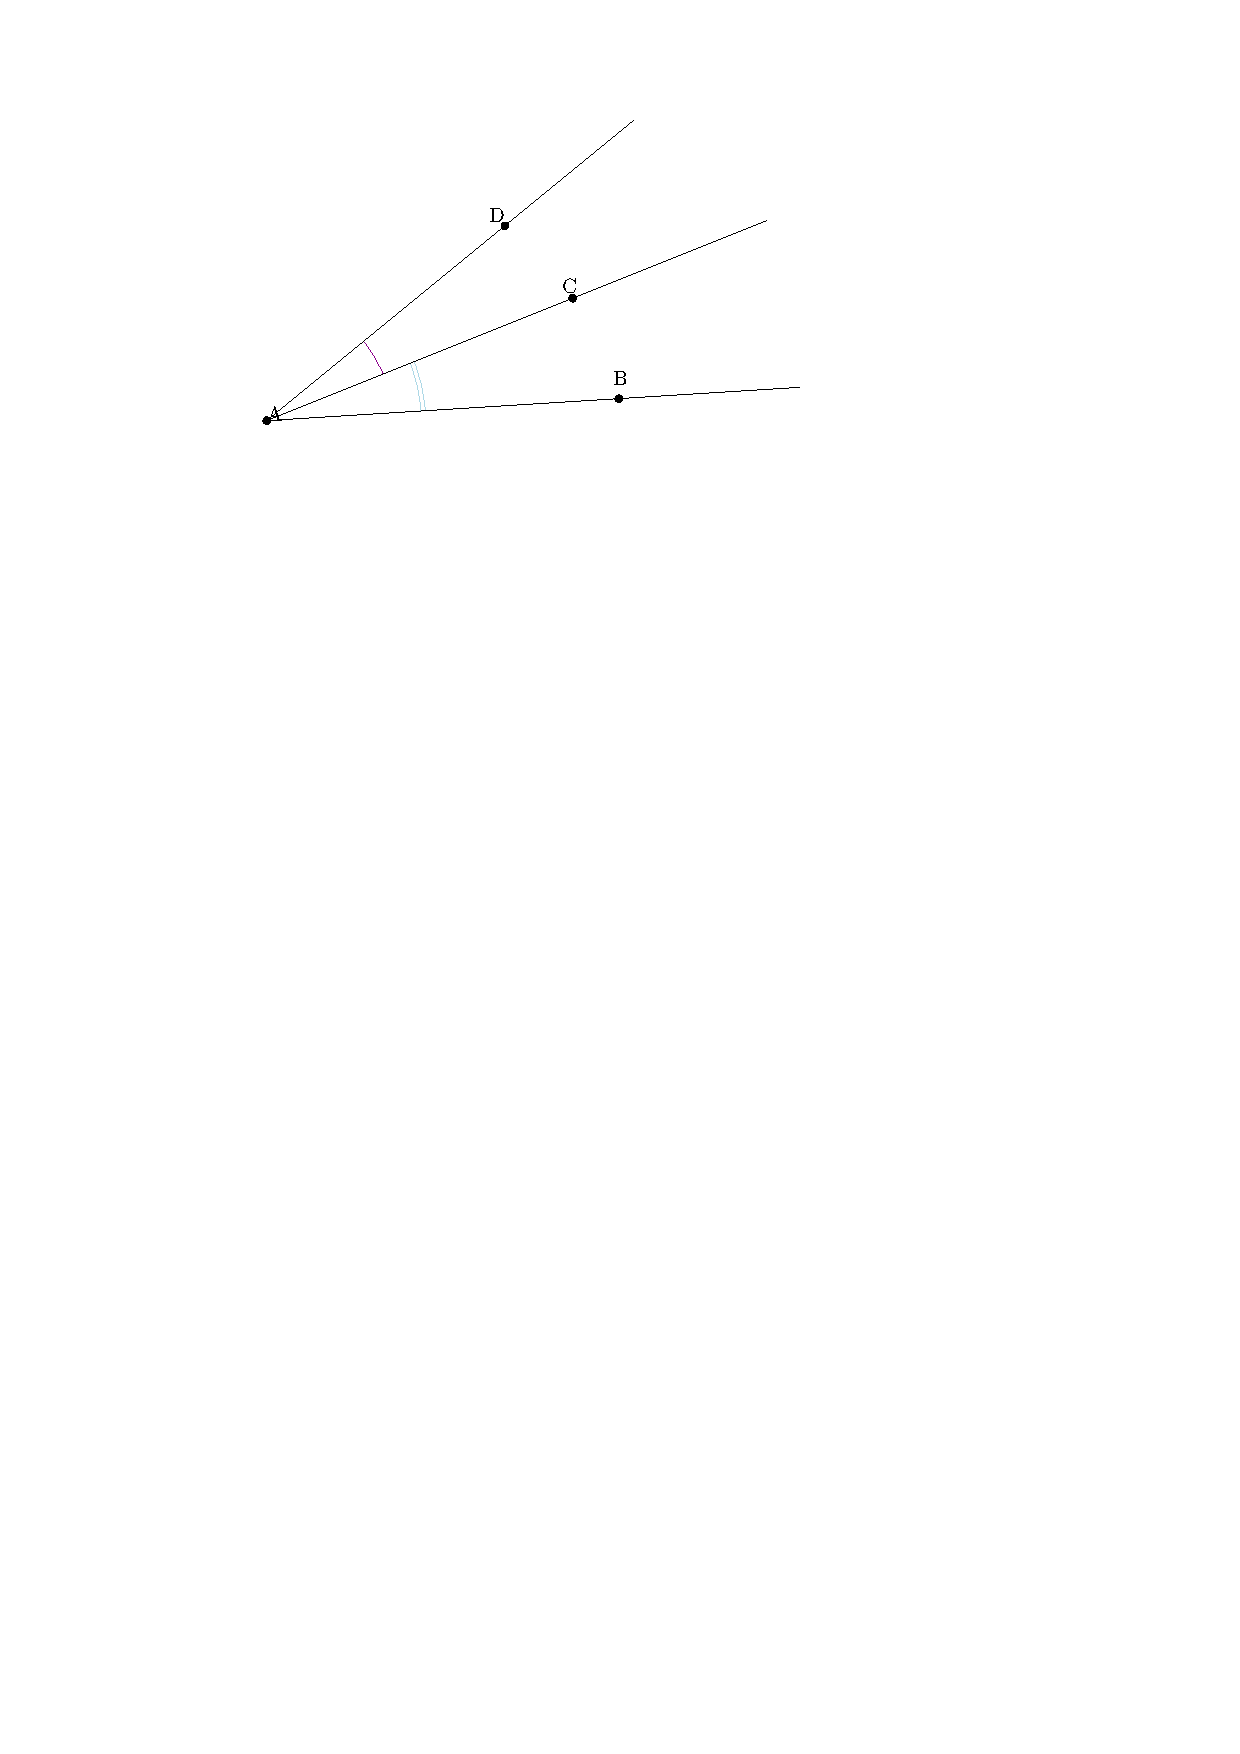
\includegraphics[width=0.8\linewidth]{5x10-angles/sources/adjacents.pdf}
  \end{figure}
\end{multicols}

\subsection*{Angles opposés par le sommet}
\begin{multicols}{2}
  \begin{Definition}{Angles opposés par le sommet}\\
    Deux angles sont opposés par le sommet si :
    \begin{itemize}
    \item Ils ont un même sommet;
    \item Les côtés de l'un sont le prolongement des côtés de l'autre.
    \end{itemize}
  \end{Definition}
  \begin{figure}[H]
    \centering
    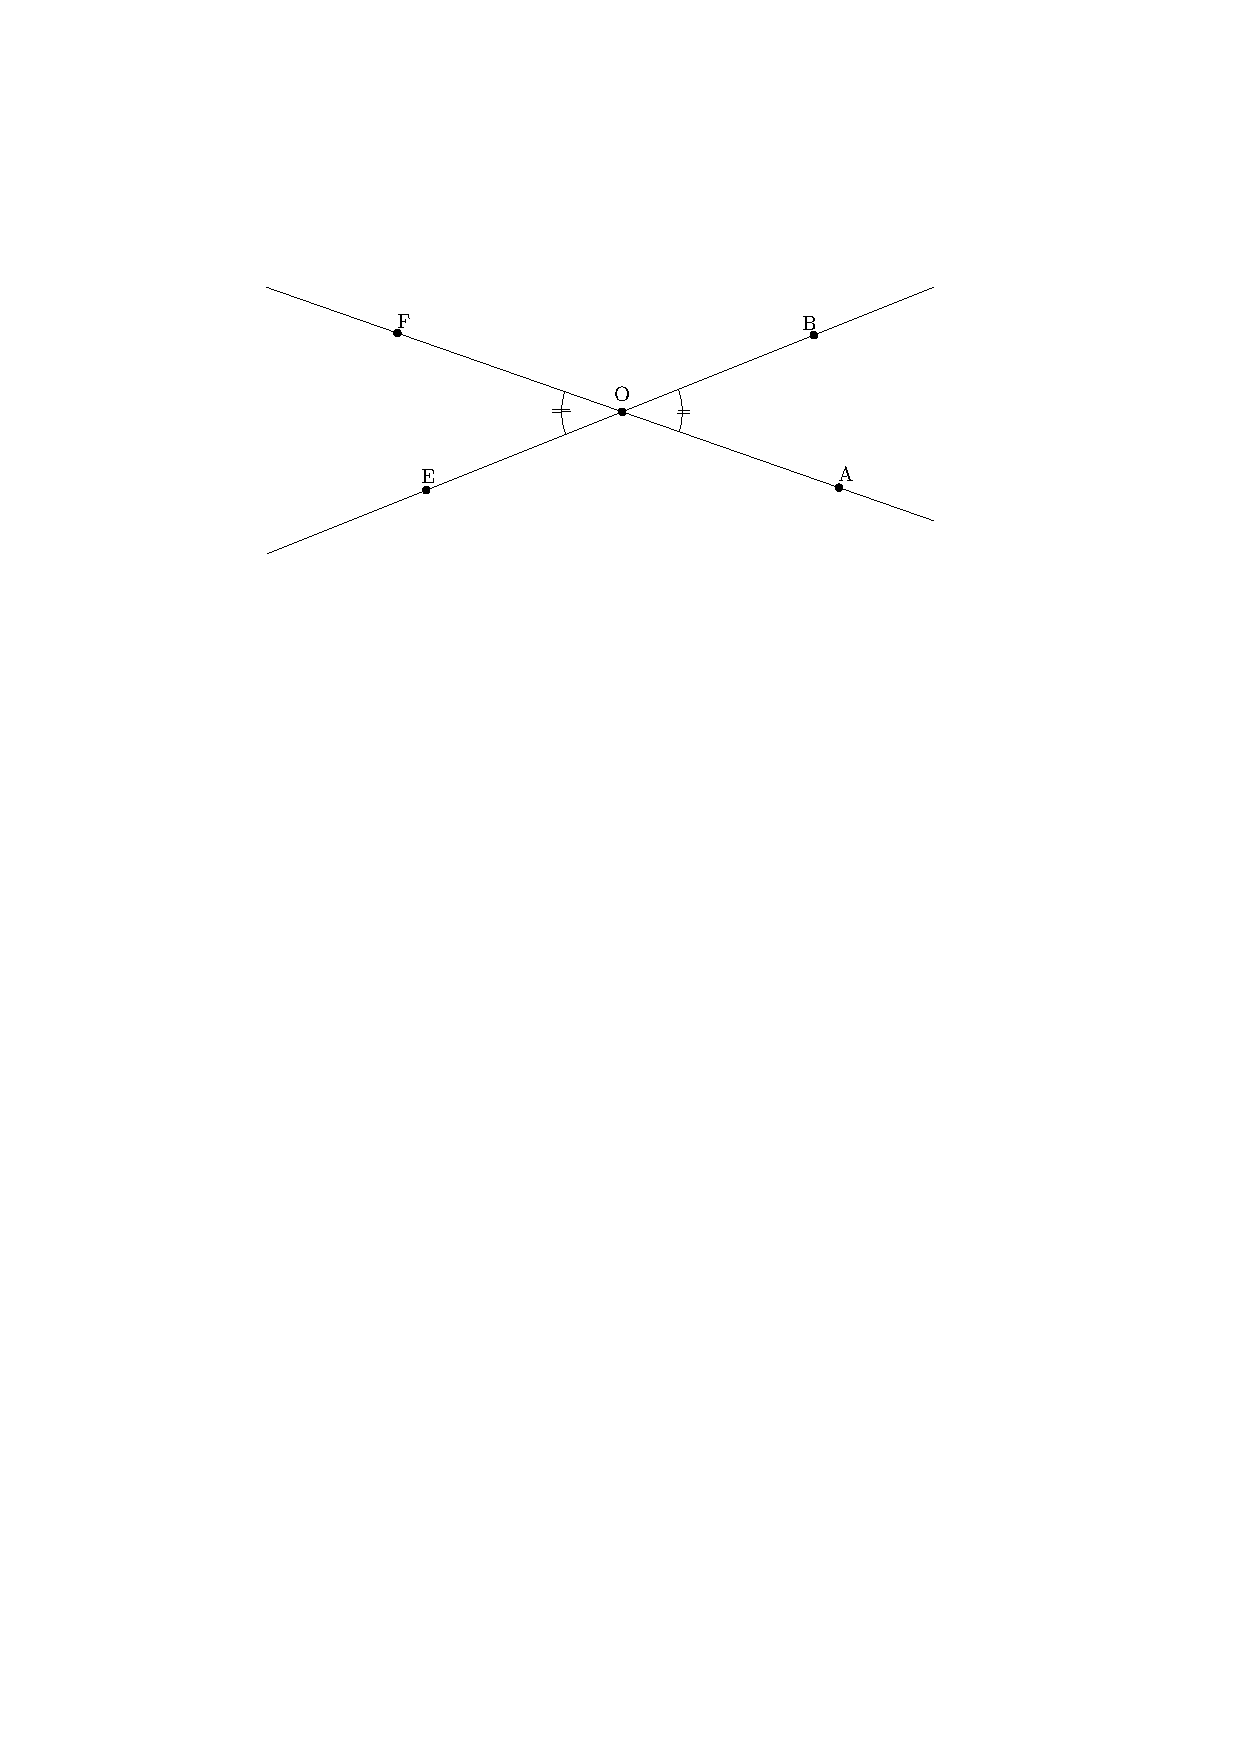
\includegraphics[width=0.8\linewidth]{5x10-angles/sources/opposes.pdf}
  \end{figure}
\end{multicols}

\begin{Proposition}
  Deux angles opposés par le sommet sont égaux.
\end{Proposition}


\subsection*{Angles complémentaires}
\begin{multicols}{2}

  \begin{Definition}{Angles complémentaires}\\
    Deux angles sont complémentaires si la somme de leurs mesures est égale à 90\char6.
  \end{Definition}
  \begin{figure}[H]
    \centering
    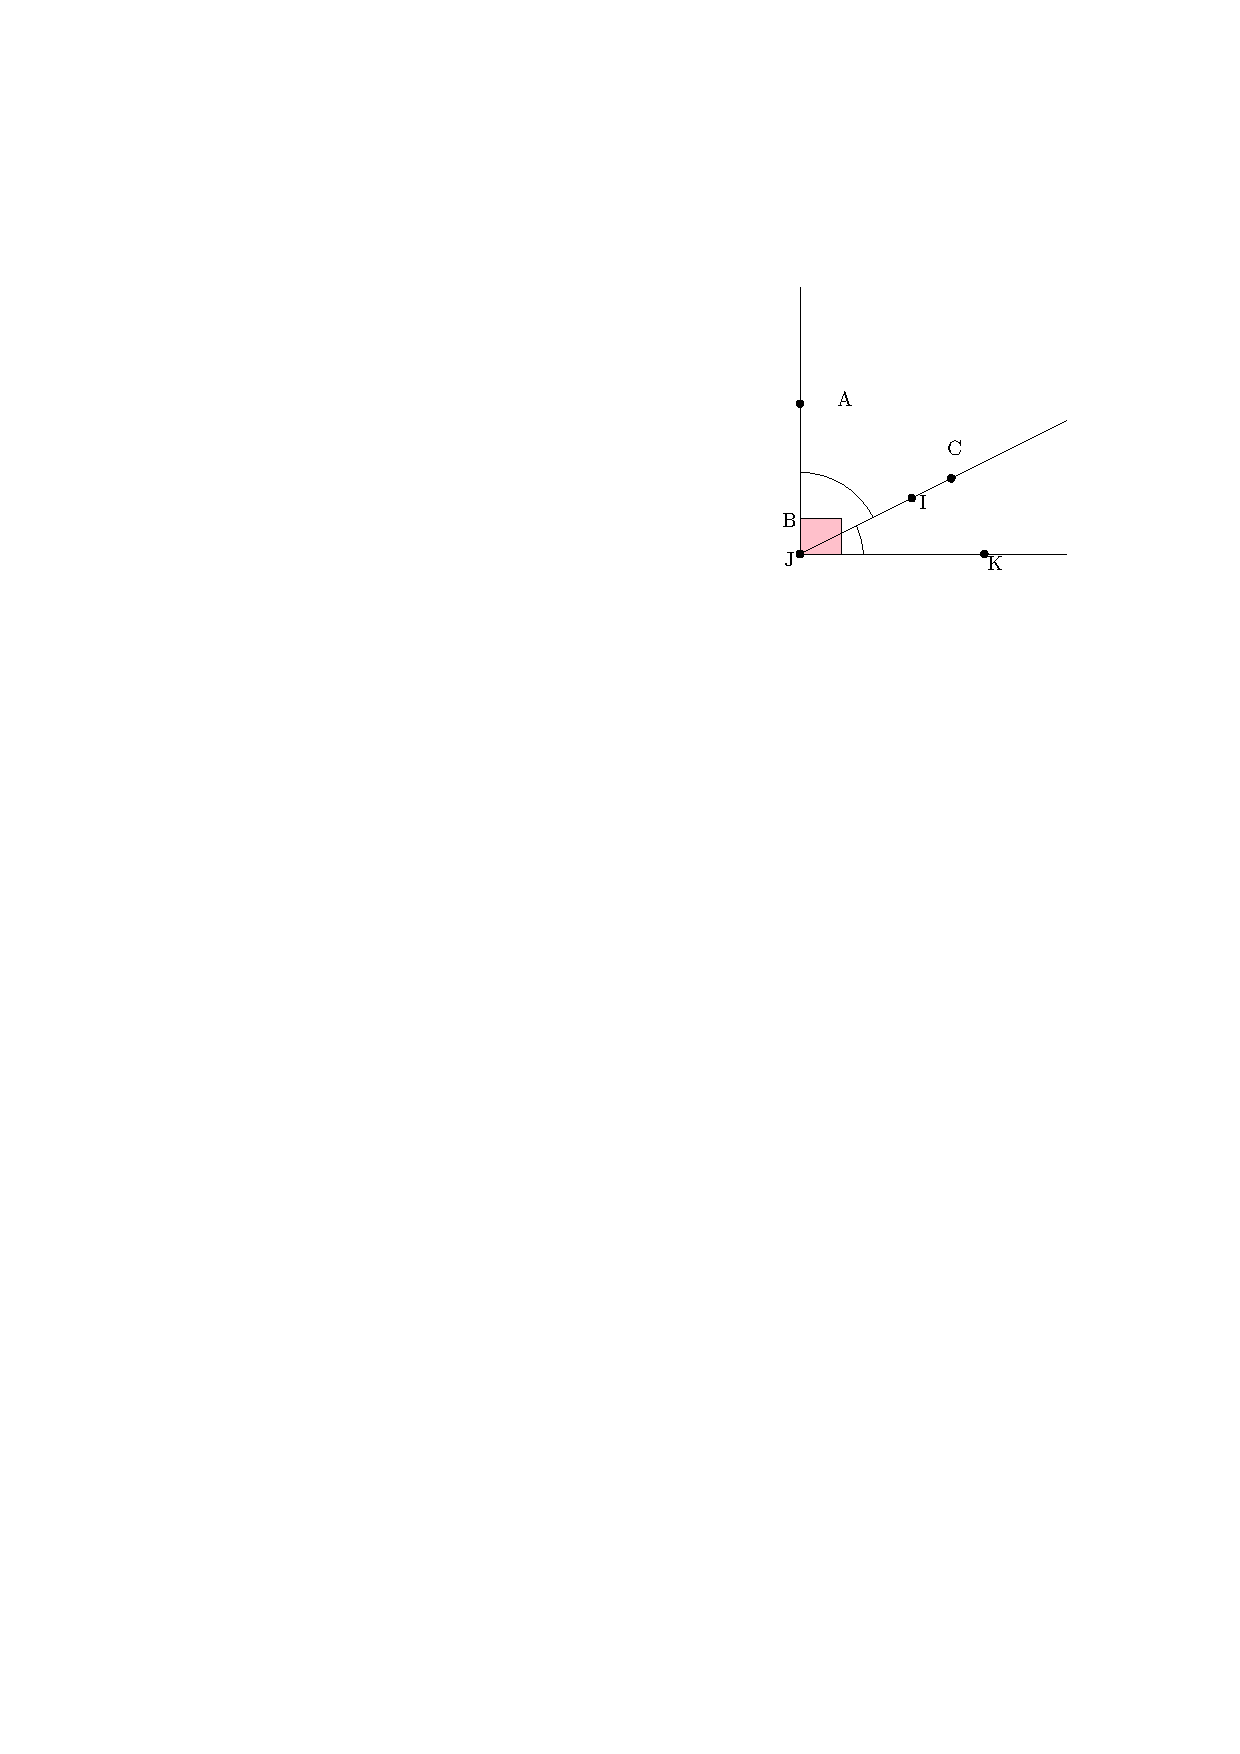
\includegraphics[width=0.6\linewidth]{5x10-angles/sources/complementaires.pdf}
  \end{figure}
\end{multicols}

\subsection*{Angles supplémenaitres}
\begin{multicols}{2}
  \begin{Definition}{Angles supplémentaires}\\
    Deux angles sont supplémentaires si la somme de leurs mesures est égale à 180\char6.
  \end{Definition}
  \begin{figure}[H]
    \centering
    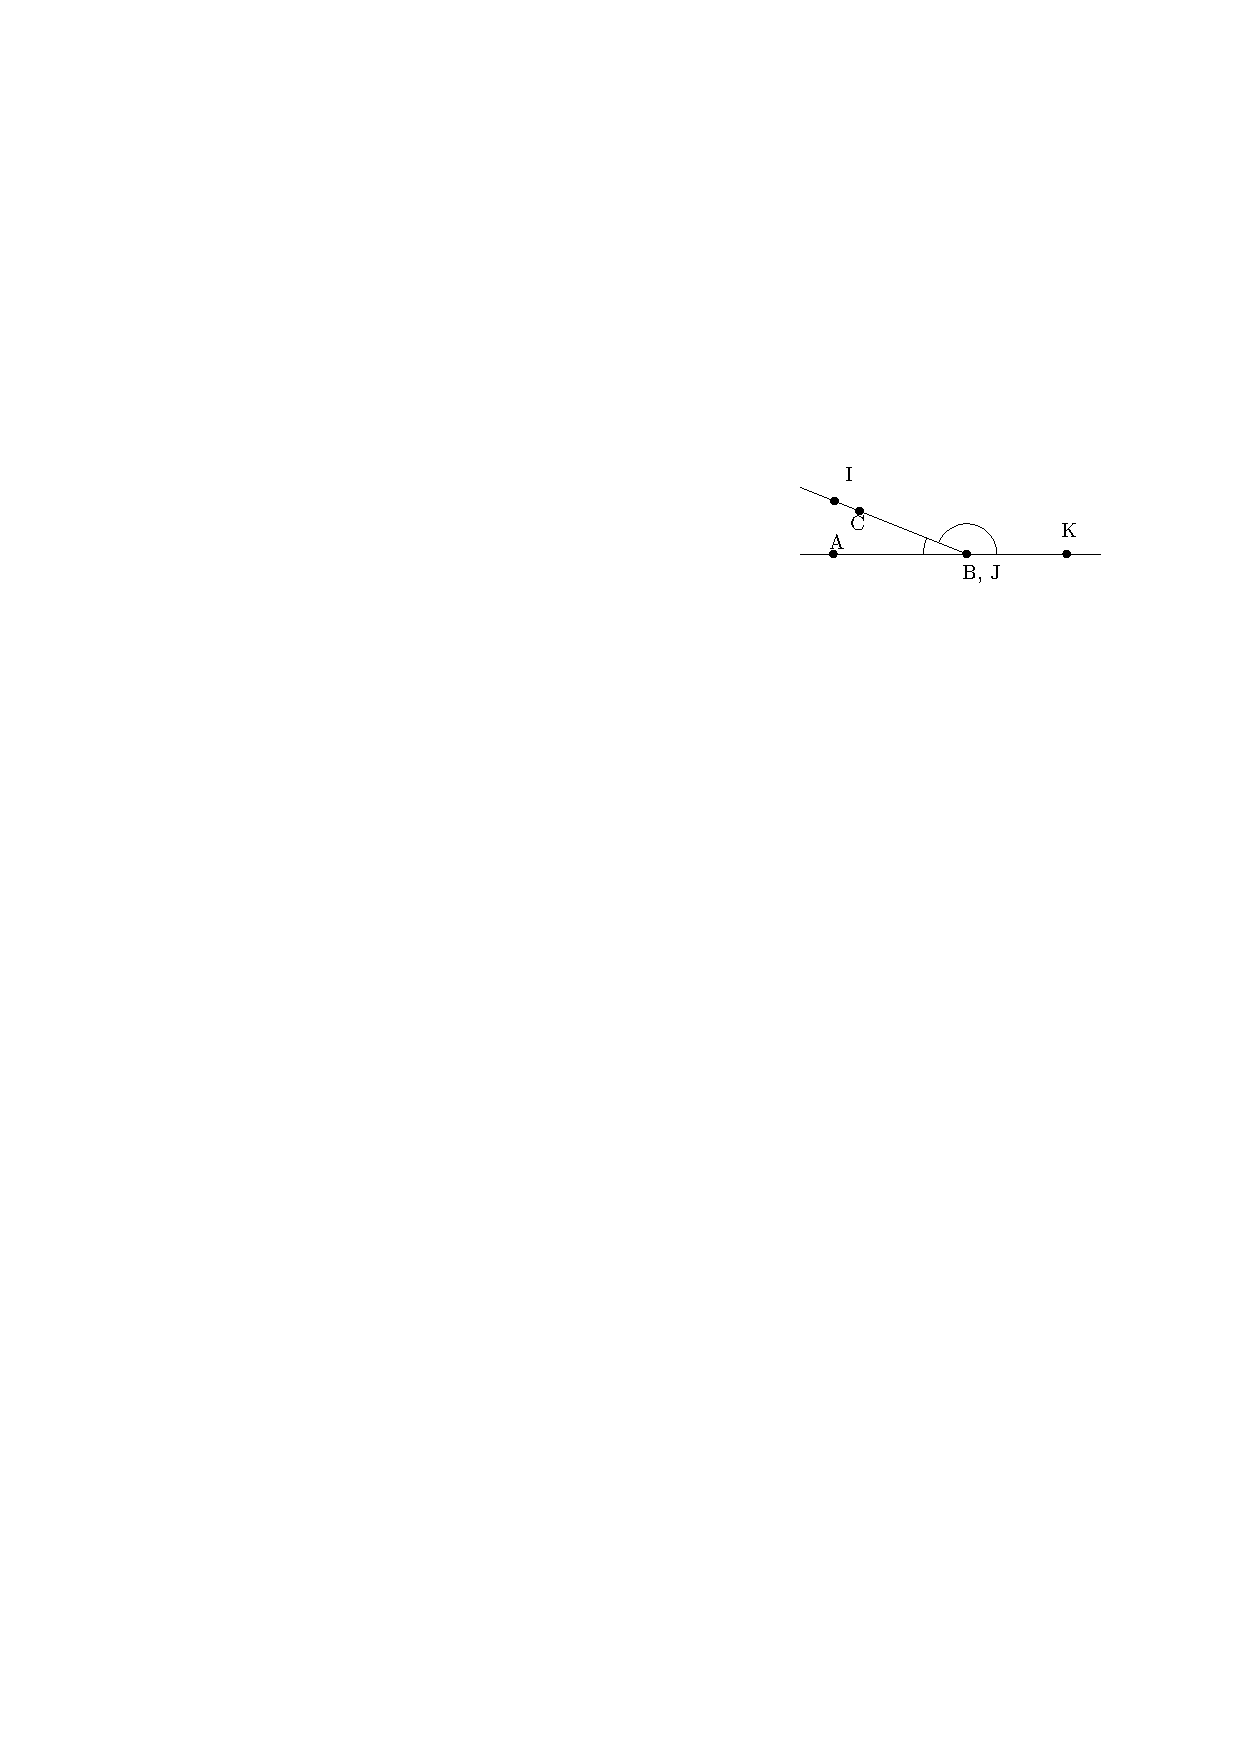
\includegraphics[width=0.8\linewidth]{5x10-angles/sources/supplementaires.pdf}
  \end{figure}
\end{multicols}


%-----------------------------------111111111111111111111111111111111111
\section*{Angles et parallélisme}
%----------------------------------------------------------------------

Soient deux droites $d_1$ et $d_2$ coupées par une troisième droite $d_3$.
\subsection*{Angles alternes-internes}
\begin{multicols}{2}
  \begin{figure}[H]
    \centering
    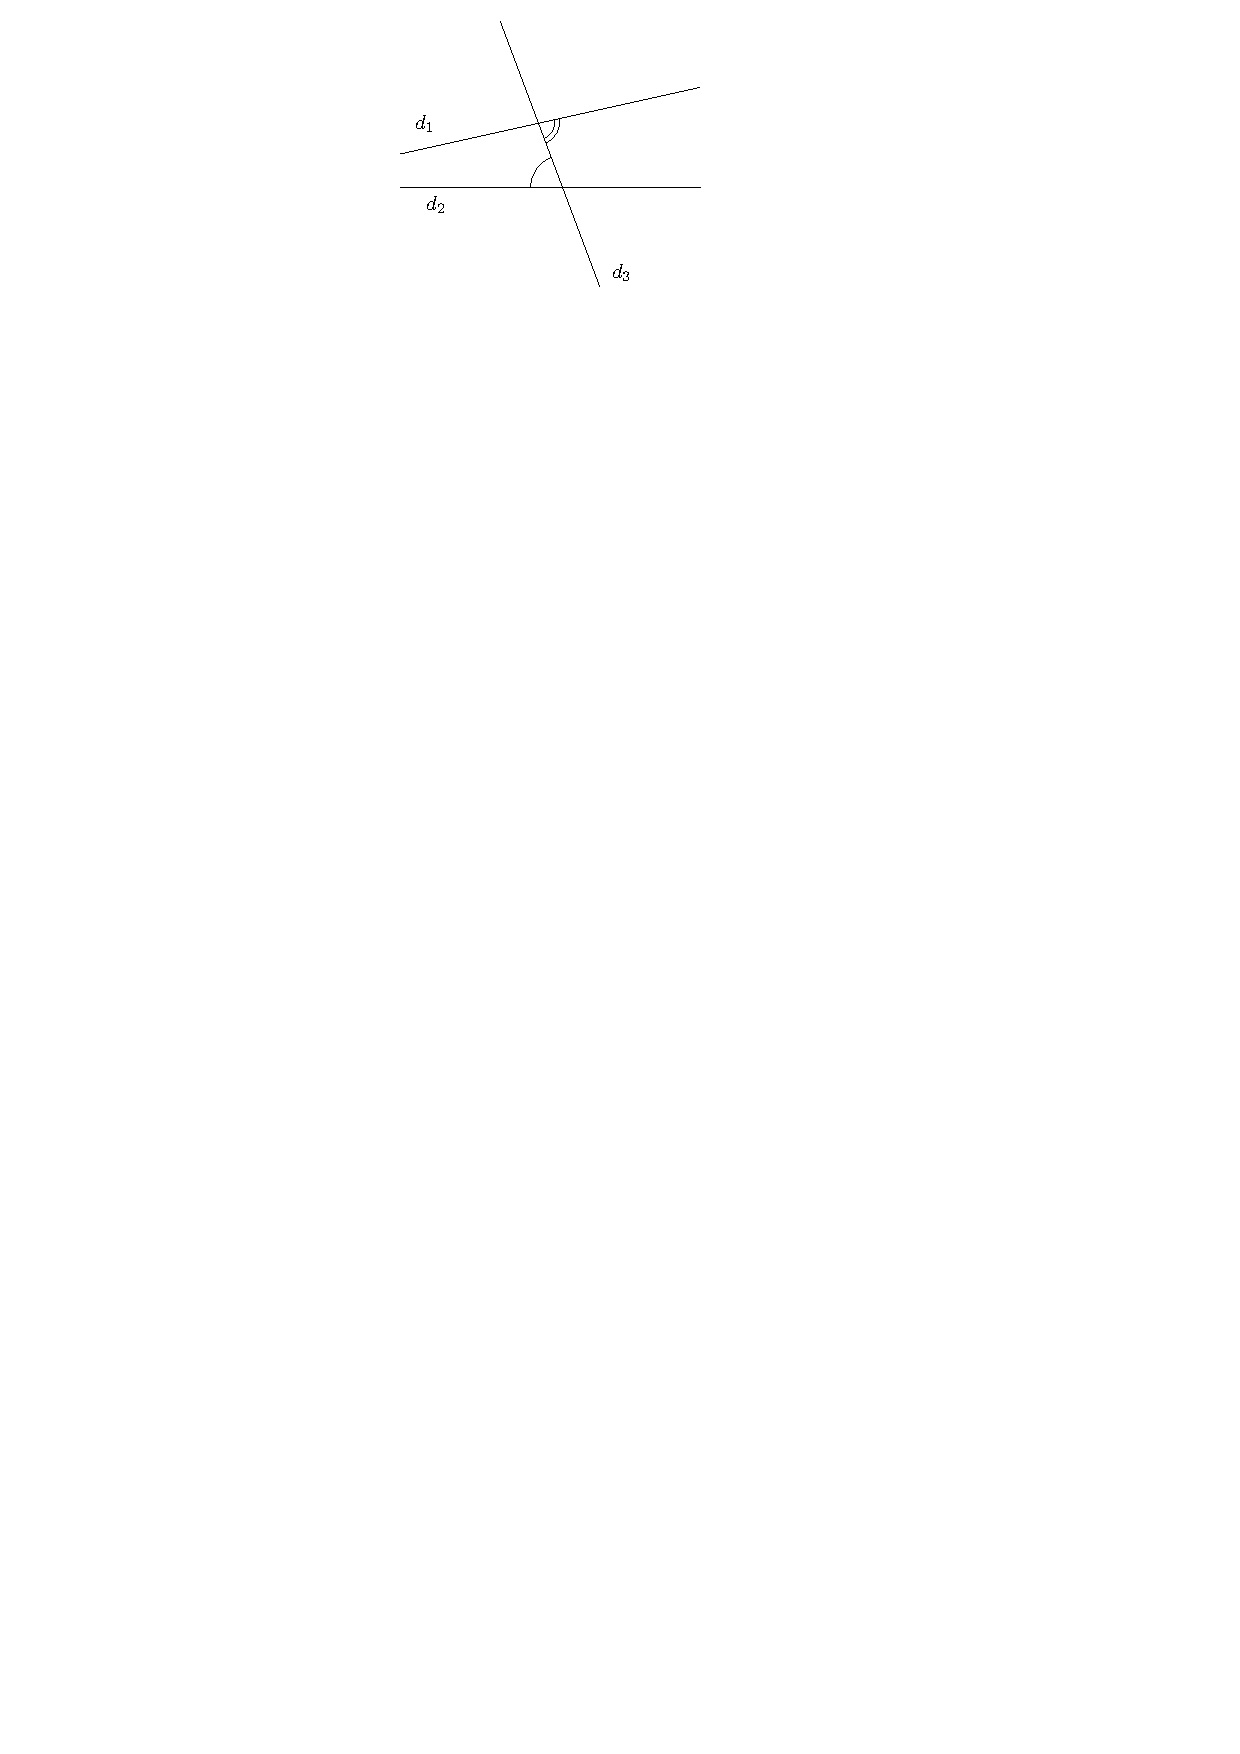
\includegraphics[width=0.8\linewidth]{5x10-angles/sources/ai-1.pdf}
  \end{figure}
  \begin{figure}[H]
    \centering
    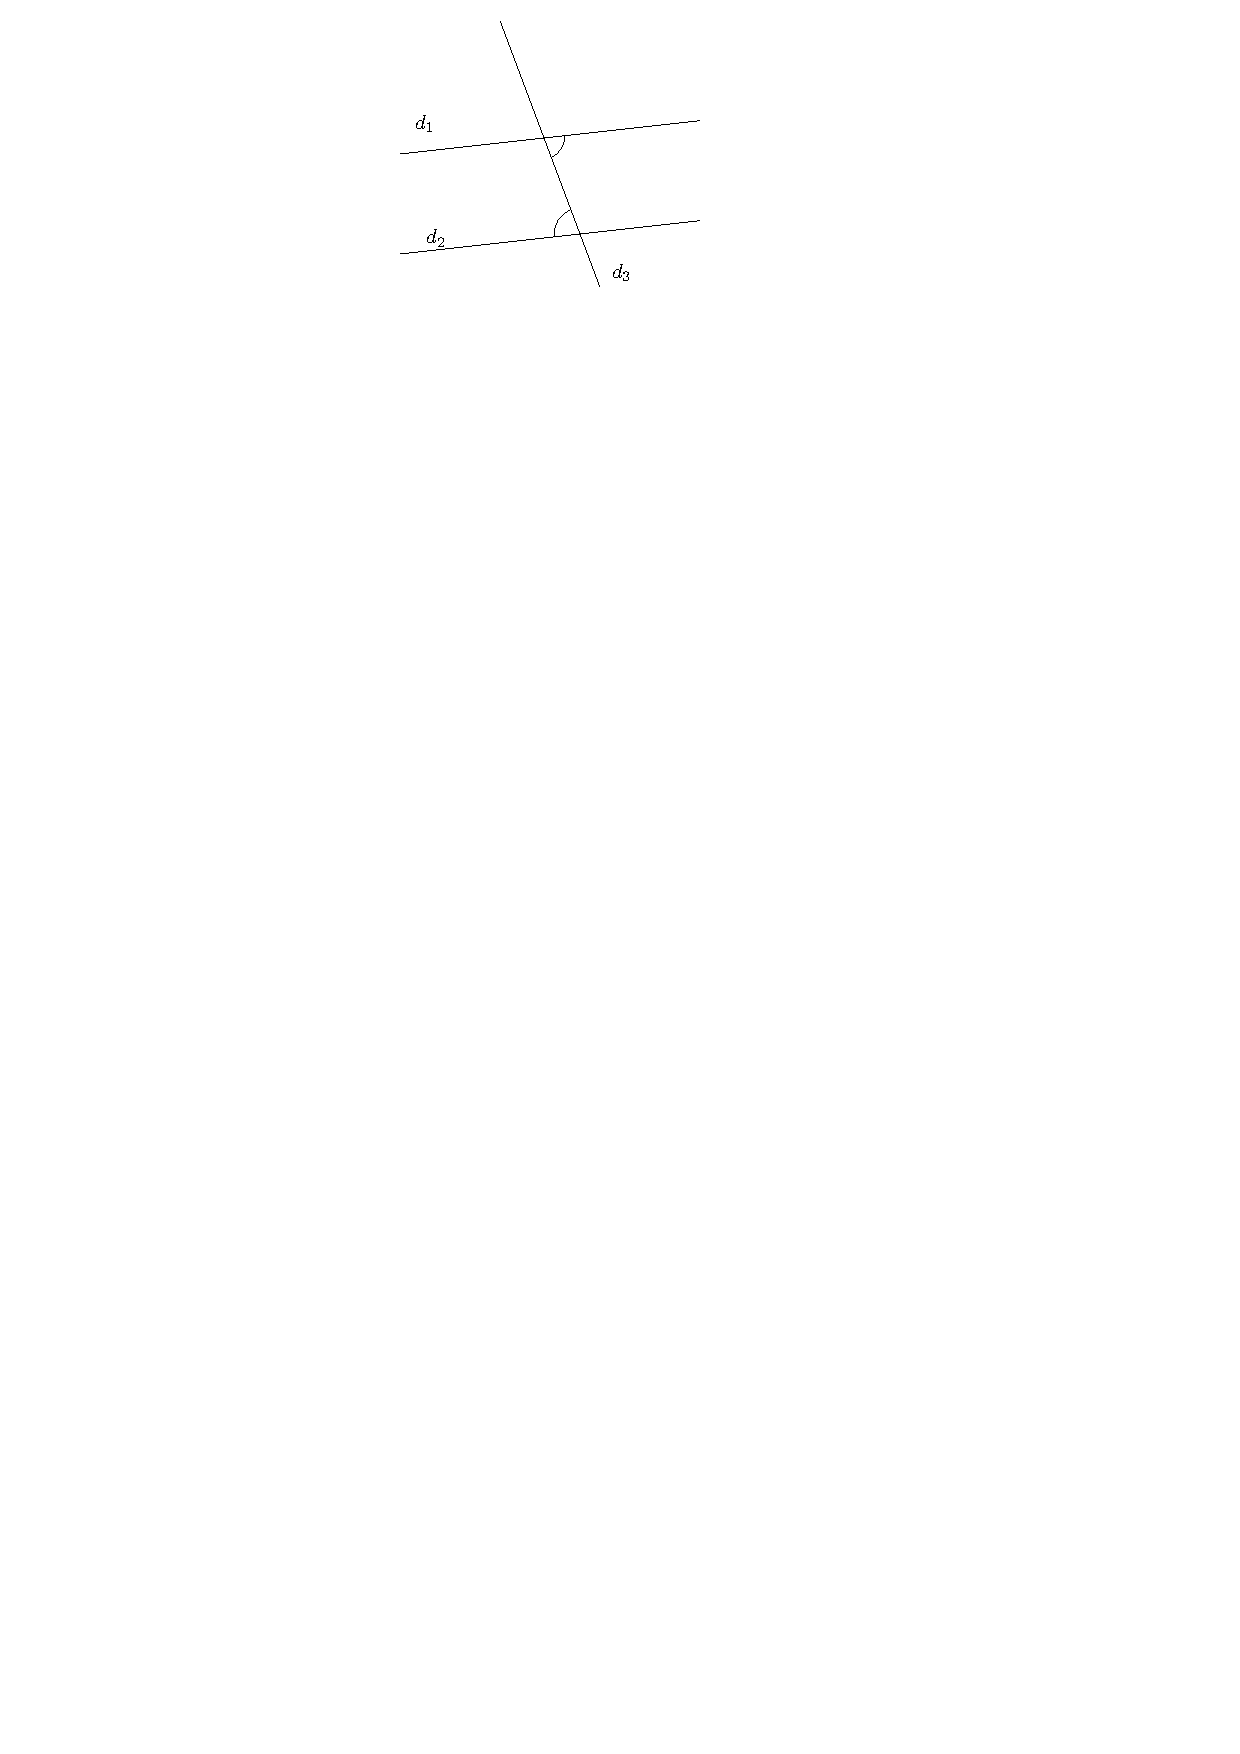
\includegraphics[width=0.8\linewidth]{5x10-angles/sources/ai-2.pdf}
  \end{figure}
\end{multicols}
\begin{multicols}{2}
  \begin{Definition}{Angles alternes-internes}\\
  \end{Definition}

  \begin{Proposition}{$d_1$ et $d_2$ sont parallèles.}\\
    Les angles alternes-internes sont égaux.
  \end{Proposition}
\end{multicols}
\subsection*{Angles correspondants}
\begin{multicols}{2}
  \begin{figure}[H]
    \centering
    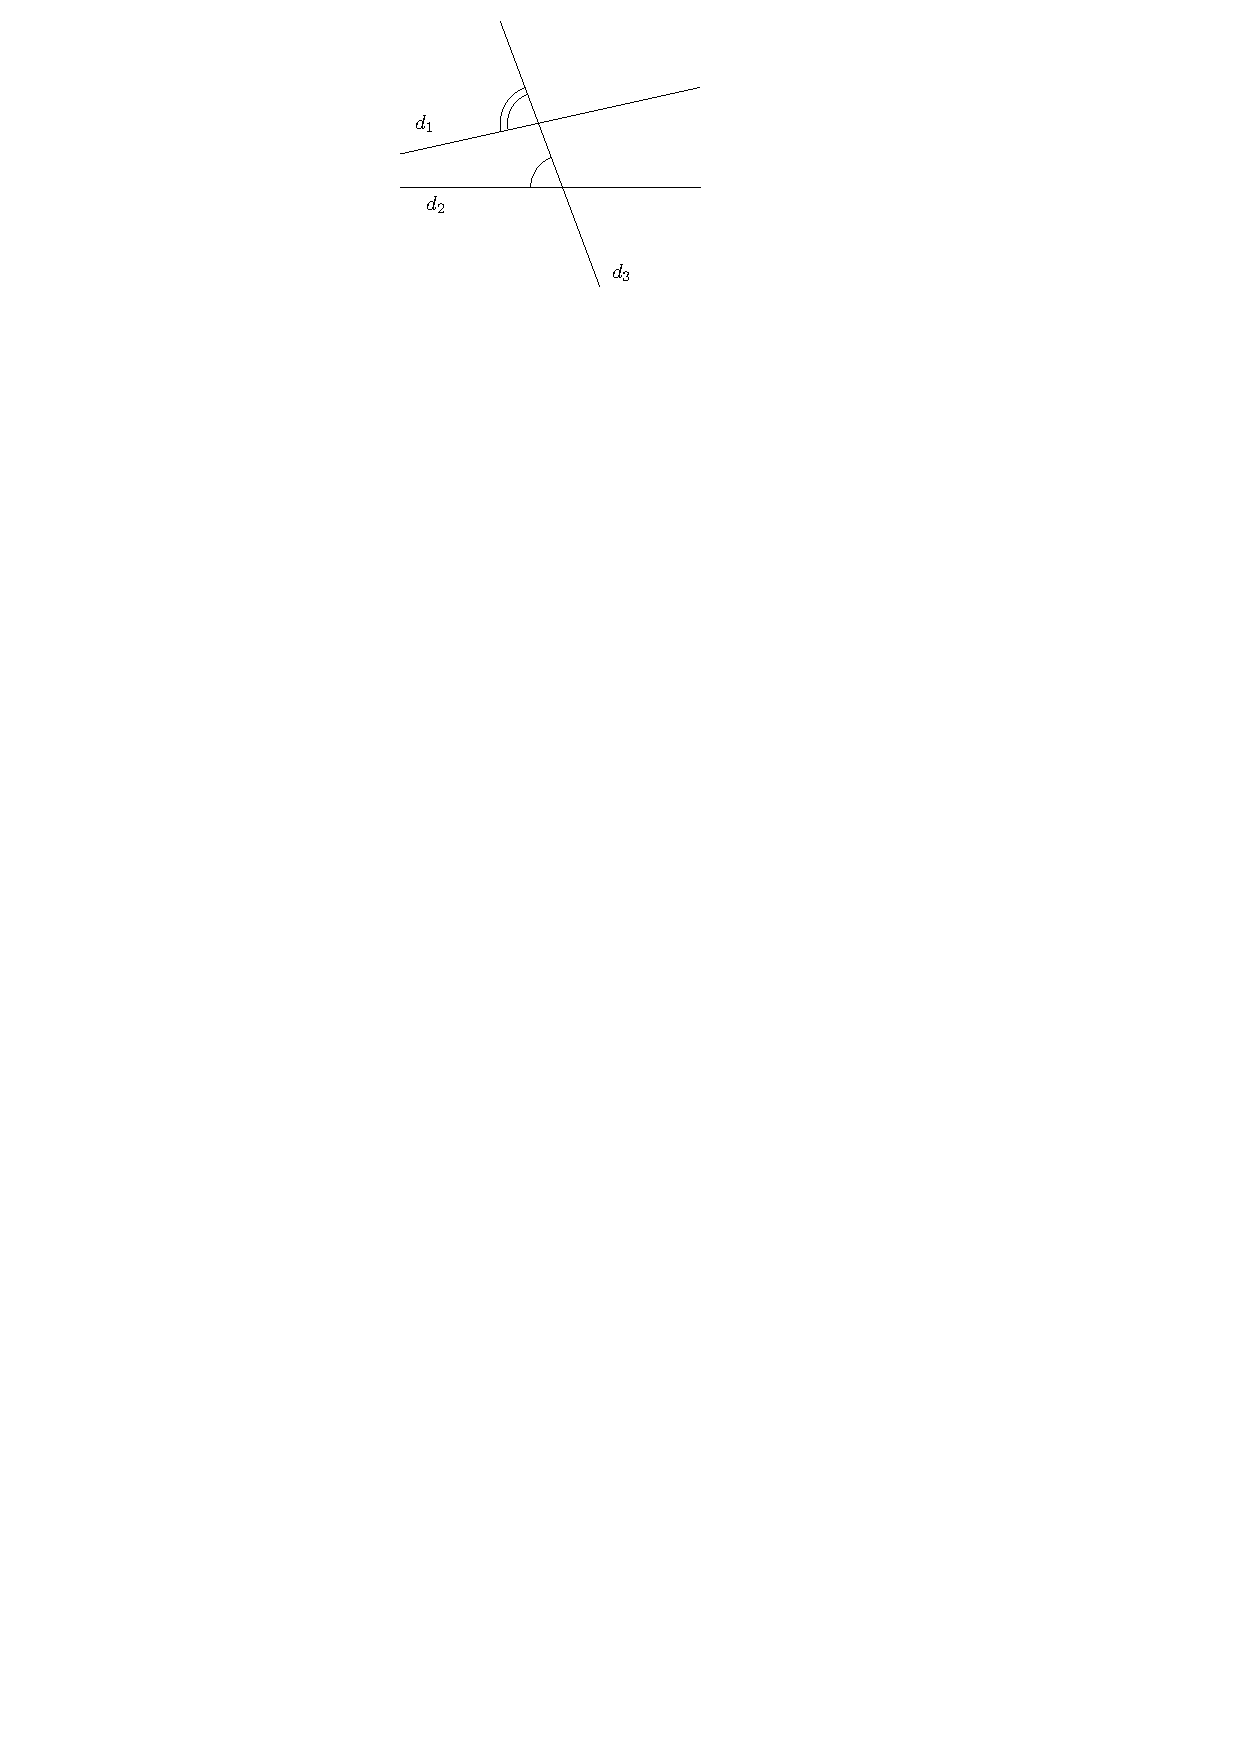
\includegraphics[width=0.8\linewidth]{5x10-angles/sources/corres-1.pdf}
  \end{figure}
  \begin{figure}[H]
    \centering
    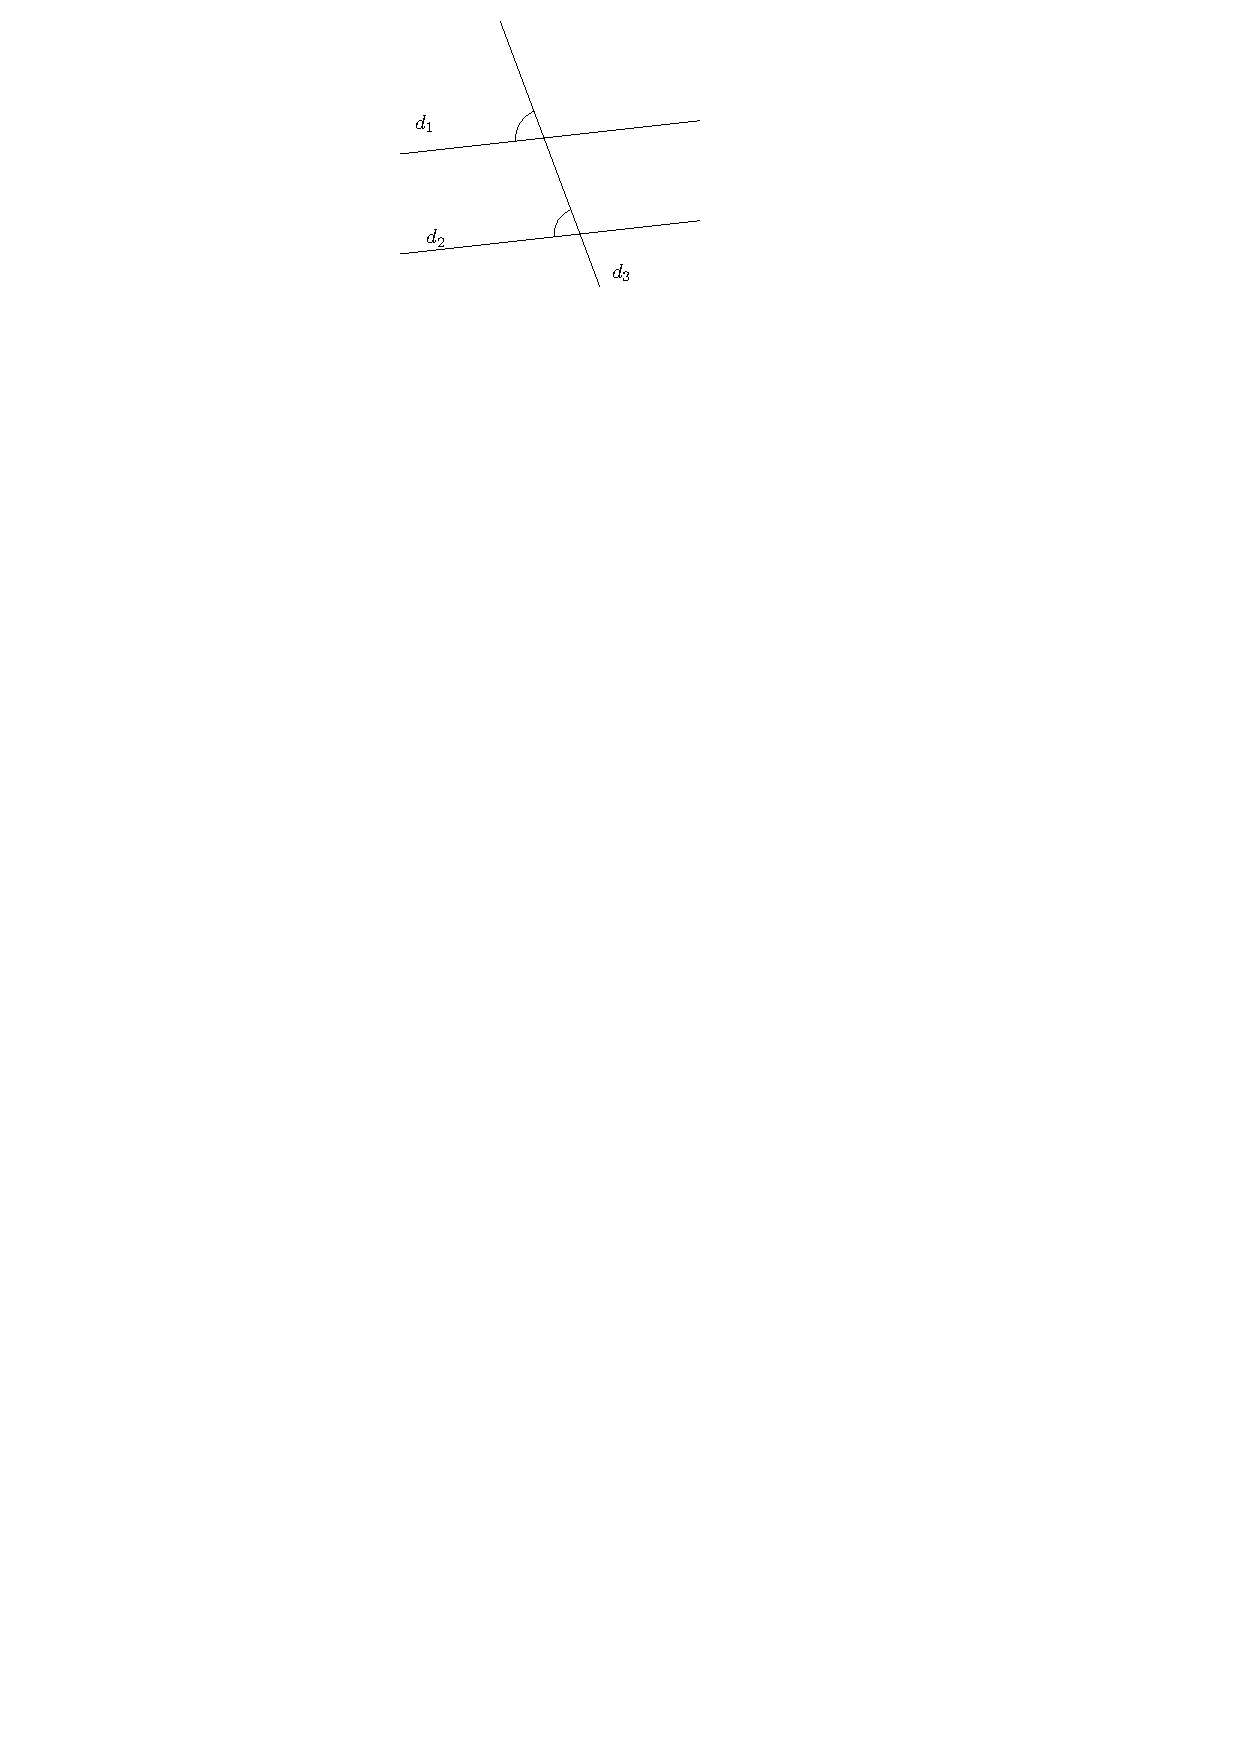
\includegraphics[width=0.8\linewidth]{5x10-angles/sources/corres-2.pdf}
  \end{figure}
\end{multicols}

\begin{multicols}{2}
  \begin{Definition}{Angles correspondants}\\
  \end{Definition}

  \begin{Proposition}{$d_1$ et $d_2$ sont parallèles.}\\
    Les angles correspondants sont égaux;
  \end{Proposition}
\end{multicols}

\end{document}
